        \documentclass{standalone}
        \usepackage{tikz}
        \begin{document}
        \fontsize{16px}{16px}\selectfont
        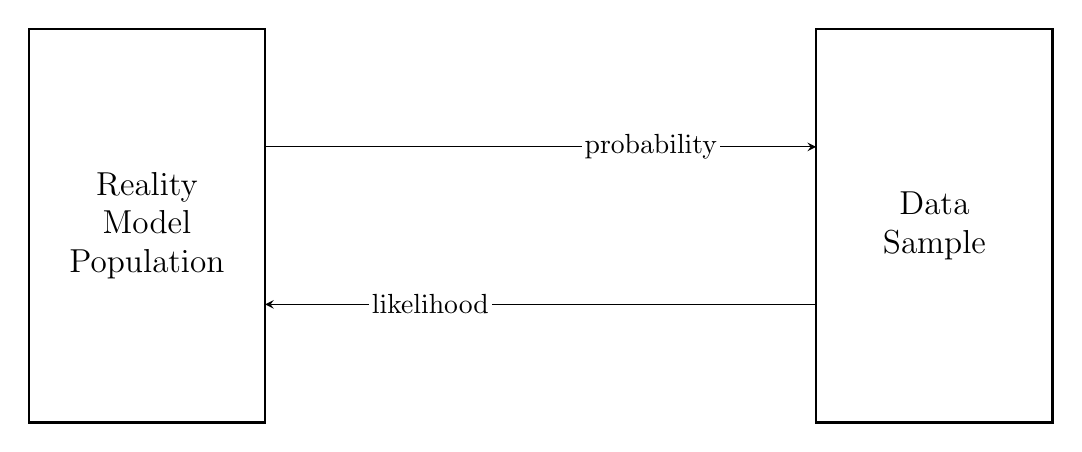
\begin{tikzpicture}

  \node (bx1) at (0,0) [draw,thick,minimum width=3cm,minimum height=5cm] {};
  \node[align=center,font=\large,rotate=0] at (bx1.center) {Reality \\ Model \\ Population};
  \node (bx2) at (10,0) [draw,thick,minimum width=3cm,minimum height=5cm] {};
  \node[align=center,font=\large,rotate=0] at (bx2.center) {Data \\ Sample};
  \draw [->,>=stealth] (1.5,1) -- node[pos=.7,fill=white,inner sep=1pt]{probability}(8.5,1);
  \draw [->,>=stealth] (8.5,-1) -- node[pos=.7,fill=white,inner sep=1pt]{likelihood}(1.5,-1) ;
        \end{tikzpicture}
        \end{document}
